\begin{frame}
  \frametitle{Turbulence Models}
  Numerous types of turbulence models exist of various turbulent flow applications. By order of
  increasing computational complexity:
  \begin{itemize}
      \item RANS-based models
      \begin{itemize}
          \item Eddy viscosity models
          \begin{itemize}
              \item Algebraic models
              \item One- and two-equation models
          \end{itemize}
          \item \gls{RSM}
      \end{itemize}
      \item \gls{DES}
      \item \gls{LES}
      \item \gls{DNS}
  \end{itemize}
\end{frame}

\begin{frame}
  \frametitle{Turbulence Models}
  \gls{RANS}-based models are based on the RANS equations obtained by applying time-averaging on
  the fluid flow equations:
  \begin{align}
      \frac{\partial U_i}{\partial t} + U_j \frac{\partial u_i}{\partial x_j} =&
      -\frac{1}{\rho} \frac{\partial P}{\partial x_i} + \nu \nabla^2 U_i -
      \frac{\partial \langle u_i u_j \rangle}{x_j}
  \end{align}
  Eddy viscosity models operate on the eddy viscosity hypothesis:
  \begin{align}
      \langle u_iu_j \rangle =& \frac{2}{3}k \delta_{ij} - \nu_T \left(
      \frac{\partial U_i}{\partial x_j} + \frac{\partial U_j}{\partial x_i}
      \right)
  \end{align}
  The various eddy viscosity models mainly differ in their approach to the closure problem of
  calculating the eddy viscosity.
\end{frame}

\begin{frame}
  \frametitle{Turbulence Models}
  Podila et al. \cite{podila_cfd_2019} found that while significant differences in turbulent
  intensities were observed near the wall, the temperature distribution did not vary significantly.
  \begin{columns}
    \column[t]{5.5cm}
  \begin{figure}
    \centering
    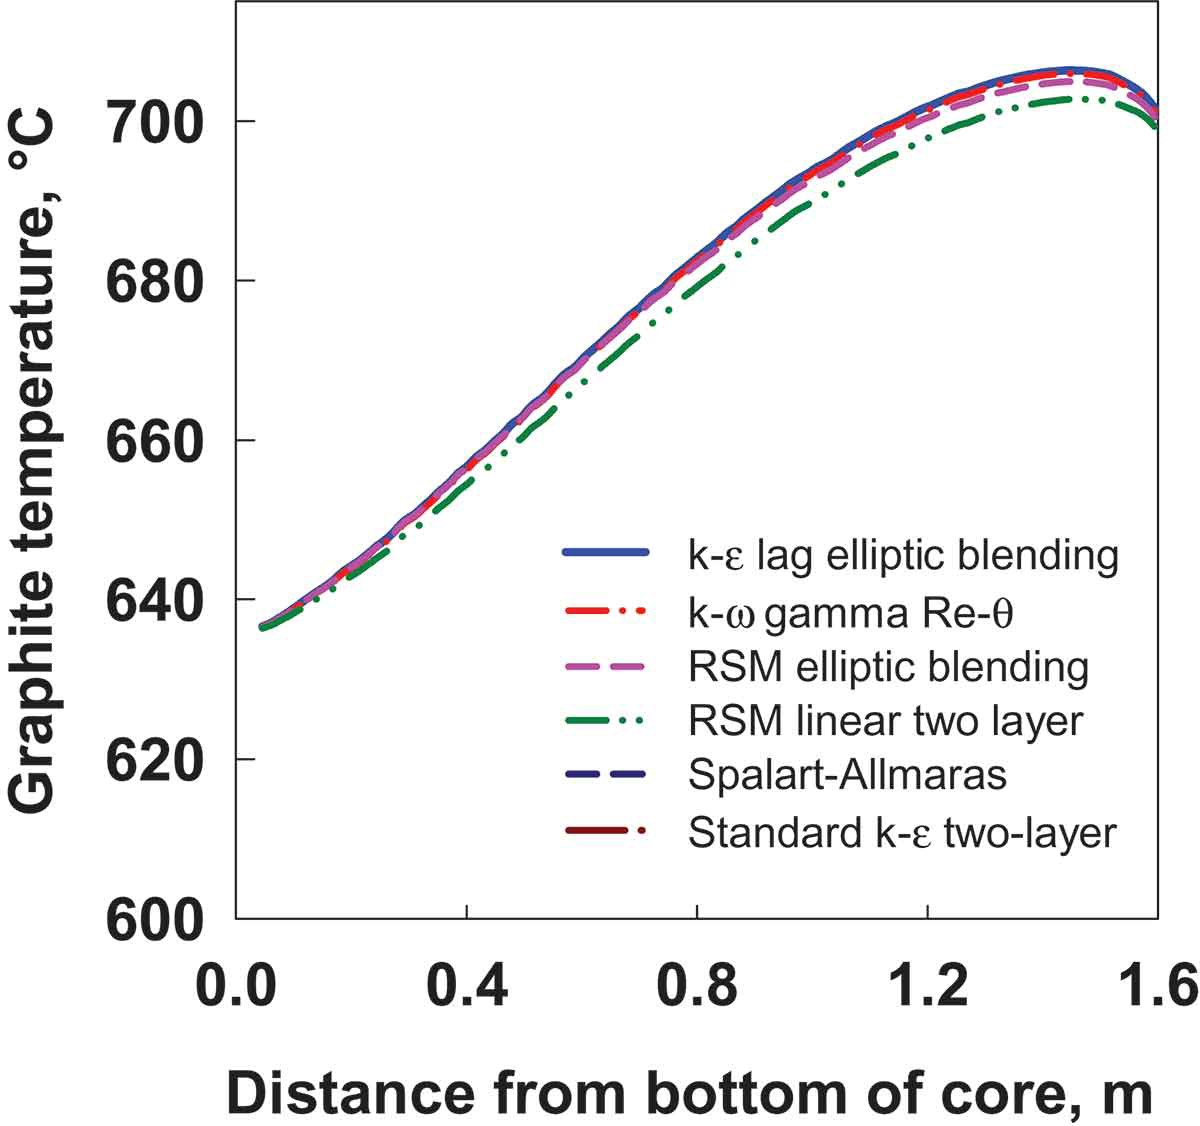
\includegraphics[width=.8\columnwidth]{images/podila-graphite}
    \caption{Graphite temperature adjacent to the hottest MSRE channel.}
  \end{figure}
  \column[t]{5.5cm}
  \begin{figure}
    \centering
    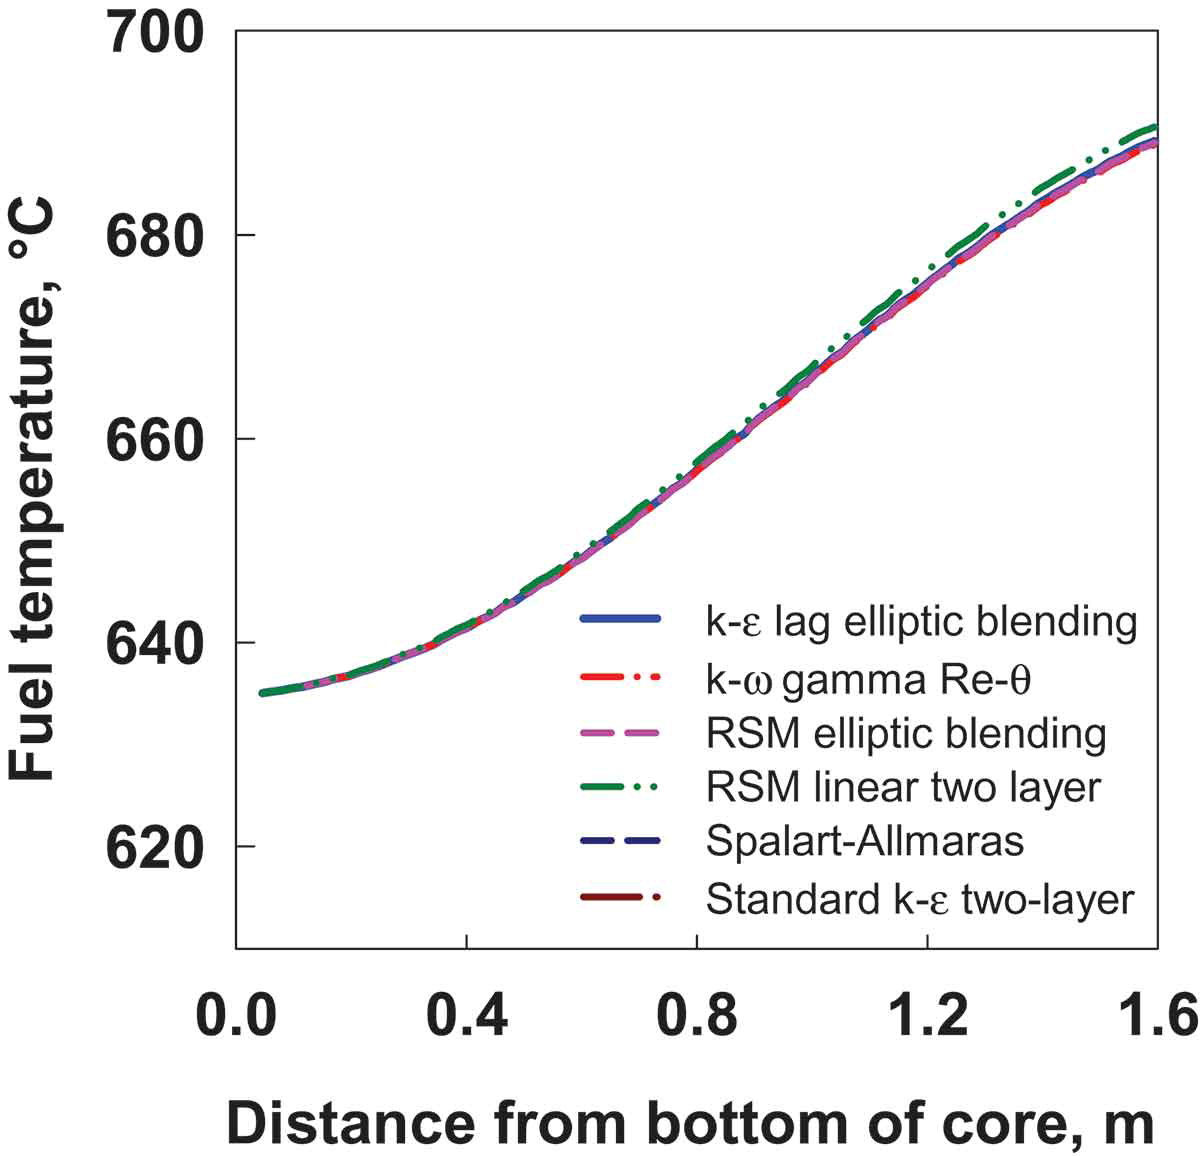
\includegraphics[width=.8\columnwidth]{images/podila-fuel}
    \caption{Fuel temperature in the hottest MSRE channel.}
  \end{figure}
\end{columns}
\end{frame}
